%!TEX ROOT=../ctutest.tex

\chapter{Dissertation plan}
\label{chap:plan}
\textit{This chapter describes my current research agenda and its meaning for my future dissertation thesis on automated fact-checking using NLP methods, which is outlined in the last section.}

\section{Automated claim generation}
\label{generation}

The article I am currently readying for submission proposes the task of \textit{automated claim generation} as the process of extracting factual claims from a textual document. It has multiple uses in practice, such as assisting the fact-checkers and emulating data for NLP tasks like automated fact-checking and NLI.

Extracting a set of factual, atomic claims from a chunk of naturally formed text poses many challenges -- what single piece of information characterizes the text best? 
How does one resolve the pronouns and coreferences in source text?
How does one adapt the extraction scheme for different speakers and stylistic forms?

I find these problems to overlap with those of the \textit{abstractive summarization} task, which has recently seen an advent of efficient solutions based on Transformer models~\cite{pegasus, brio}.

The summarization scheme only requires minor tweaks -- preventing it from outputting more than one sentence of output per input and training it on data appropriately chosen to promote the summarization of more than one fact when sampling different claims from the same model using the top-$k$\footnote{Each output token is sampled from the $k$ most probable words in the dictionary} and top-$p$\footnote{Each token is sampled from the most probable words which have at most $p$ total probability mass}~\cite{topp} strategies.

An initial training data is derived from XL-Sum~\cite{xlsum}, \FEN and \CTK, and models are trained using mBART, Pegasus, T5~\cite{t5-11b}, and LLaMA-2 (QLoRA) architectures.  Additional experiments are being carried out using the GPT Chat API.

Moving forward, the primary tasks will be a cyclic iteration of claim generation data and models, refining each part after progression in the other, and most importantly, a set of reliable metrics that are explainable and correlate with human judgment.
As shown in section~\ref{benchmarking-sota}, the standard automated summarization metrics are not appropriate as a benchmark for the task.

\section{Claim generation metrics}
\label{metrics}

\begin{figure}
    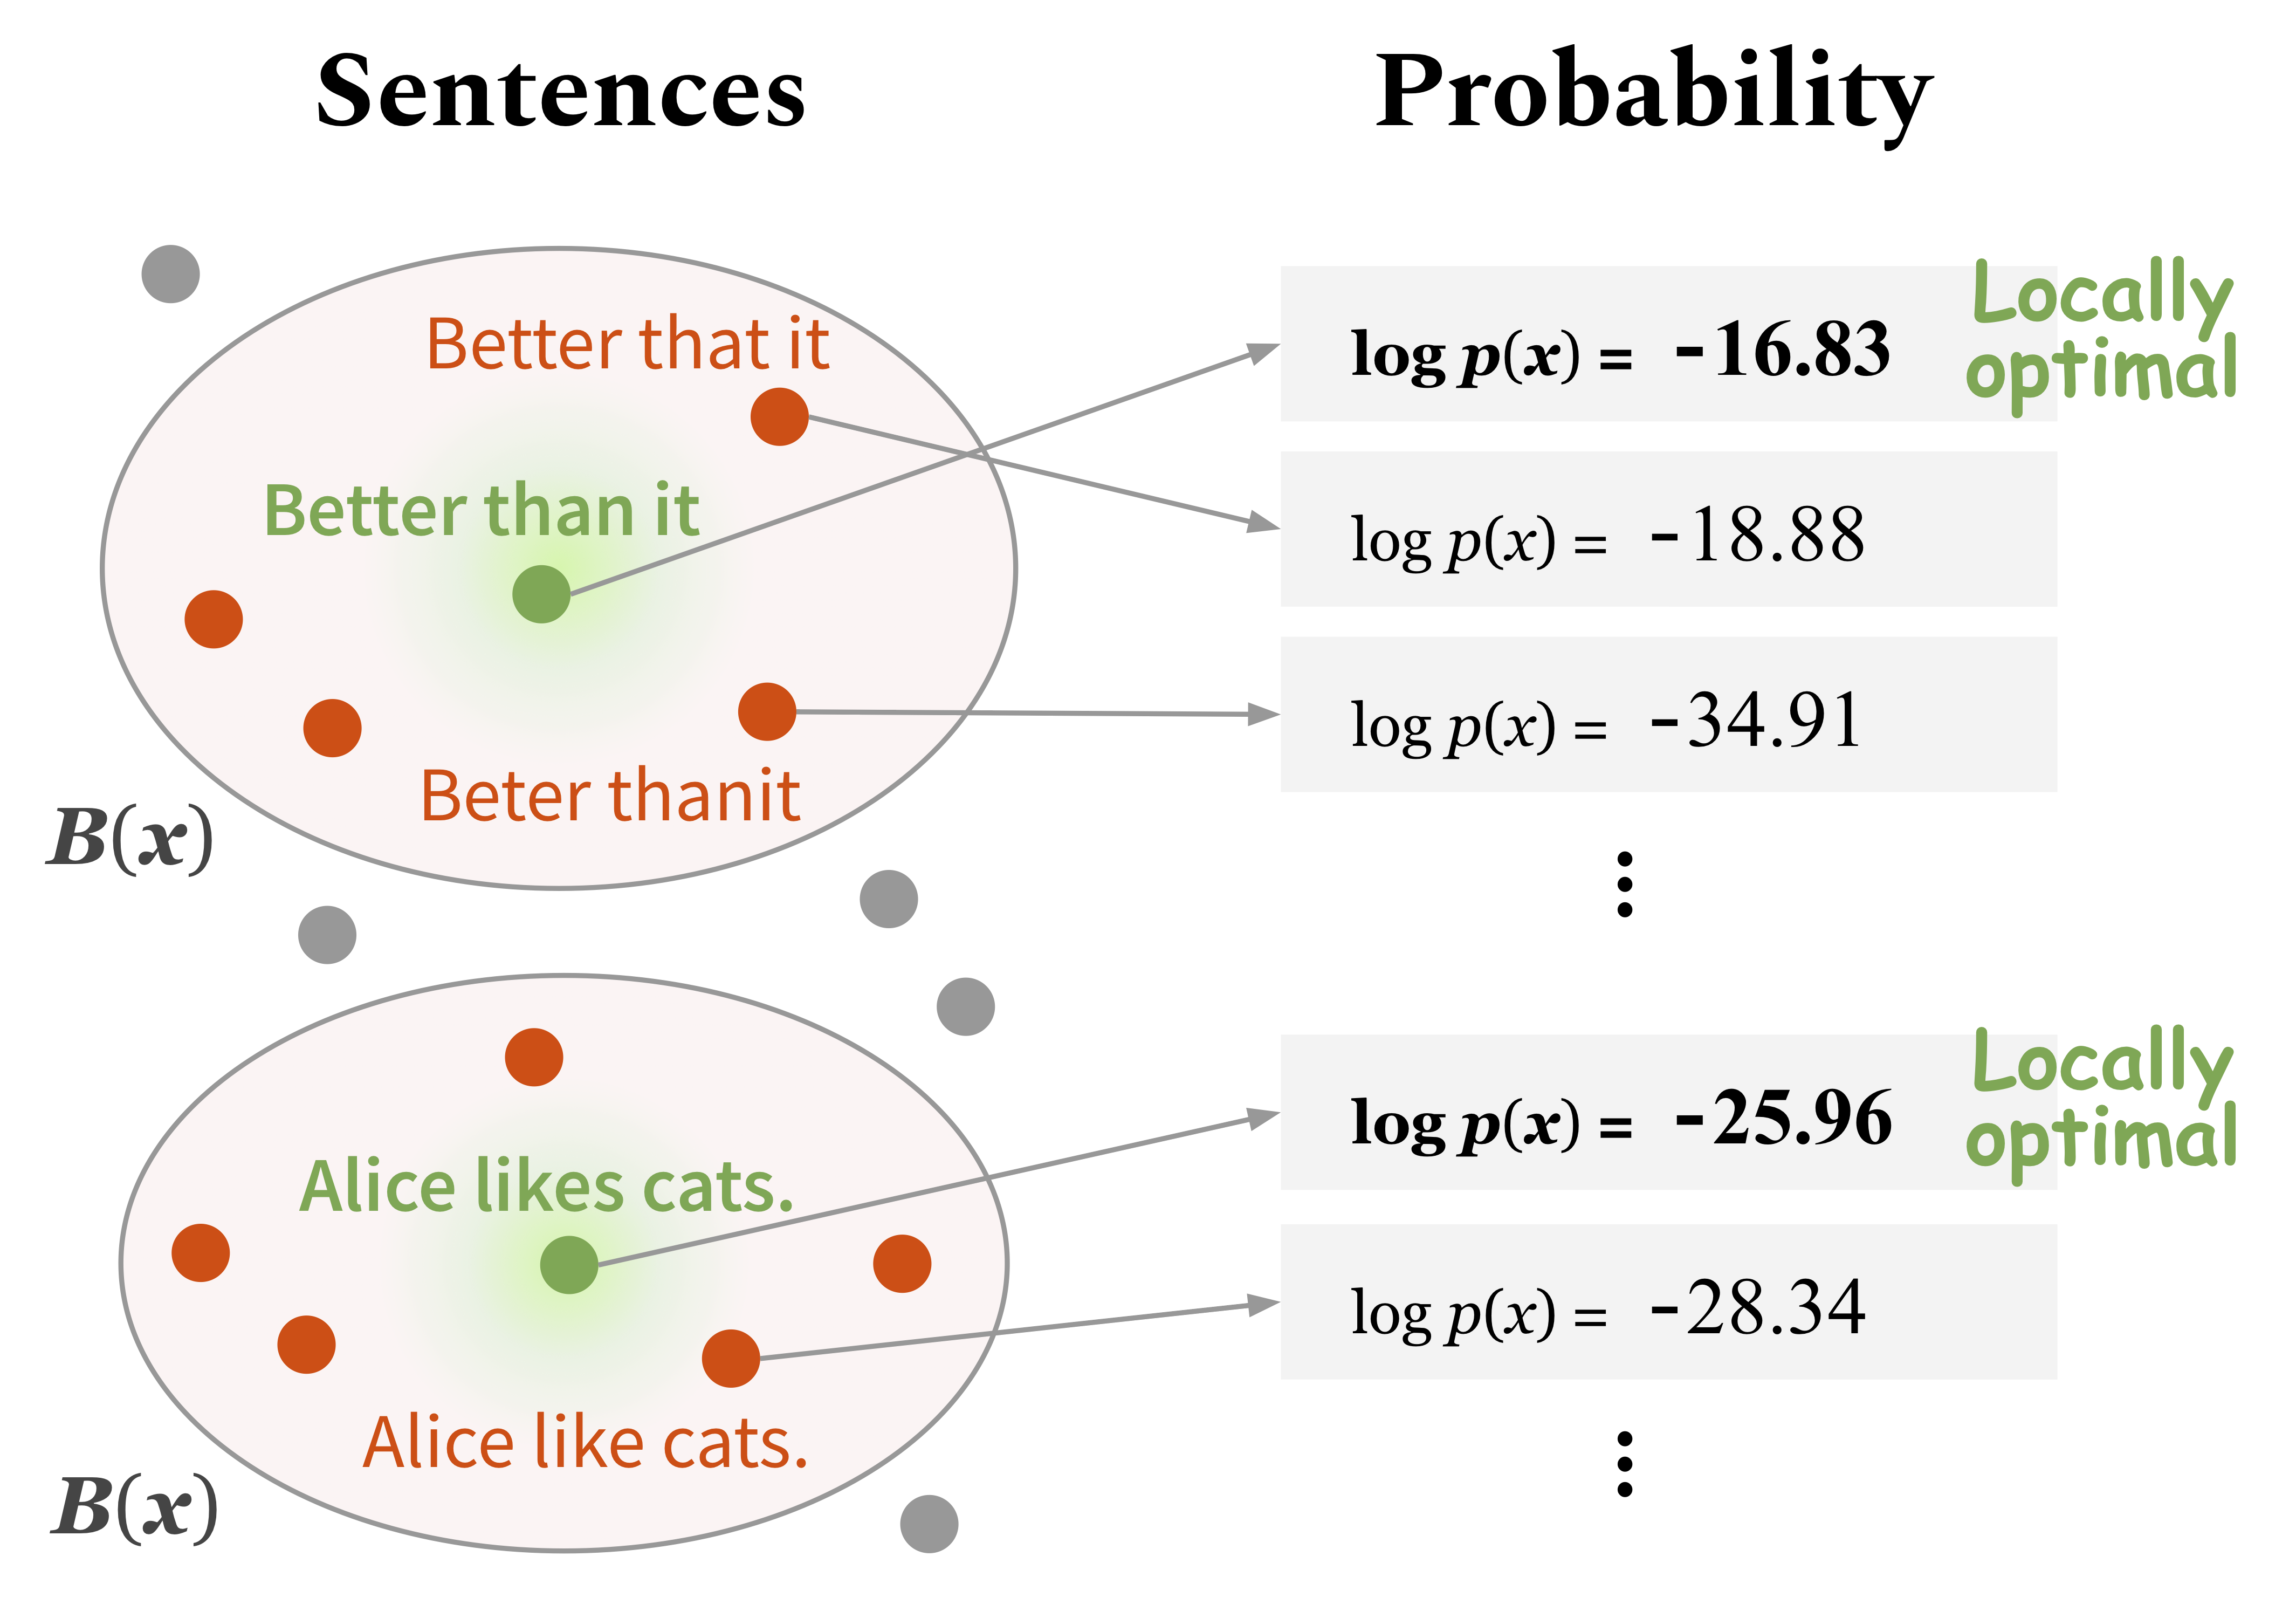
\includegraphics[width=7cm]{fig/lm_critics.png}
    \caption{\textsf{LM-Critic} -- deciding text fluency viewed as finding local optima of Language Model output probability, reprinted from~\cite{yasunaga-etal-2021-lm}}
    \label{fig:lmcritic}
\end{figure}
\label{sec:metrics}

\begin{figure}
    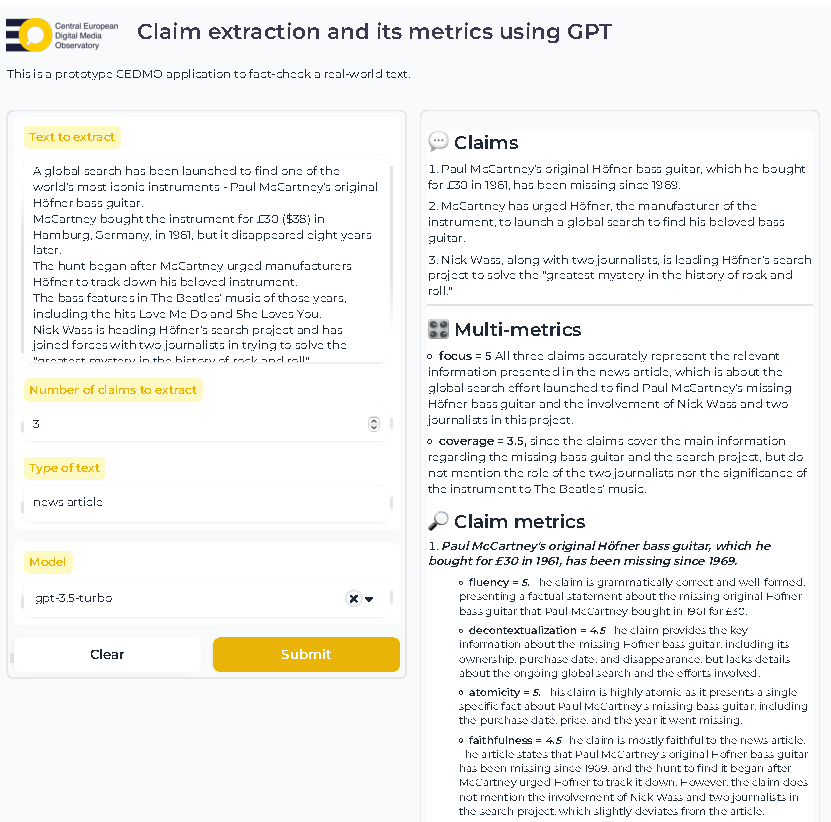
\includegraphics[width=11cm]{fig/gptext.pdf}
    \caption{A self-evaluating claim generation model based on GPT-3.5-turbo and GPT-4~\cite{gpt4} using the \textsf{OpenAI API} and a single-shot (one gold example given) approach}
    \label{fig:gptext}
\end{figure}
\label{sec:metrics}
The common problem with generative tasks in NLP is that of explaining model reasoning in a human-understandable manner and troubleshooting the prediction faults, such as the \textit{model hallucination}.

For the task of claim generation, where we also face the challenge of the \textit{relevance} of the information extracted by the model, we suggest the use of the following metrics rooted in the current research on similar topics:

\begin{enumerate}
    \item {\techbf Fluency} -- \textit{is the claim grammatically correct and intelligible?}
    
    Currently, we are working with two emulations of claim fluency, challenge that is similar to a standard NLP task of Gramatical Error Detection (GED): \textsf{LM-Critic} (Figure~\ref{fig:lmcritic})~\cite{yasunaga-etal-2021-lm} perturbs the claim words and characters to find local optima in output probability of its tokens, using a language model such as GPT-2 as its reference. \textsf{GPTScore}~\cite{fu2023gptscore} uses prompting a LLM (such as GPT-3) to obtain a model-inferred score using few- or zero-shot learning.
    
    Both can be adapted for Czech and the latter is demonstrated in Figure~\ref{fig:gptext}.
    \item {\techbf Decontextualization} -- \textit{can the claim be correctly interpreted without any additional context from the source document or elsewhere?}
    
    A common problem with machine-extracted factual claims is reusing excerpts from source documents along with inexplicable contextual pronouns (\"{President won't sue \textit{them}}) and relative referencing (\"{\textit{Last year}, CTU had 23K students}).

\cite{choi-etal-2021-decontextualization} proposes decontextualization as a sequence-to-sequence task with two texts on input $(s,c)$ -- sentence and context.
    T5 model~\cite{t5-11b} is then trained on machine-generated gold data from Wikipedia to output sentence $s^\prime$ such that the truth-conditional meaning of $s^\prime$ in an empty context is the same as that of $s$ in $c$.

    \cite{mohri2023learning} improves upon this, altering the problem formulation to minimization of surrogate loss, rejecting with a fixed predictor, and claiming to get as close as $\sim3\%$ away from the theoretical limit for the task.

    The approaches are reproducible using the Czech Wikipedia corpus and appropriate for further examination.

    \item {\techbf Atomicity} --  \textit{does the claim describe a single entity, relation or process?}
    \label{atomicity}
    
    Claim atomicity can be checked using the Relationship Extraction methods such as LUKE~\cite{yamada2020luke}. Simply put, the RE task is to identify the entities of a text (persons, institutions,\dots) and the relations between them (such as $(\textit{\"{study at}}, \textit{Herbert}, \textit{CTU})$). The atomicity evaluation can be converted to a RE task by attempting to extract such fact triples and mark the claim as atomic if there is at most one such triple found (after removing symmetries)

    \item {\techbf Faithfulness} -- \textit{does the claim only contain information that is consistent with the source document?}
    
    This metric is crucial to pinpoint \textit{model hallucinations} -- parts of the claim where the model outputs stray from the information present in the source text and begin to just \"{make stuff up}. We proceed to use two alternative metrics -- a score proposed within the FFCI evaluation framework~\cite{ffci} as: 
    $$\text{AvgTop-}n_{s_j\in X, t_i\in Y^\prime}(\textsc{BERTScore}(t_i,s_j))$$
    Where the $\text{AvgTop-}n$ simply averages across the top $n$ (say, 5) highest scores, $X,Y^\prime$ are the sets of sentences in the source document and model output, respectively (so, in the claim generation scenario $|Y^\prime|=1$) and $\textsc{BERTScore}$~\cite{bert-score} is a recently popular similarity score between two sentences that doesn't compare the texts on a verbatim level (like, e.g., ROUGE~\cite{lin-2004-rouge} which correlates poorly with human judgment) but expresses the sentence similarity as a sum of cosine similarities between their tokens' embeddings -- this should capture semantical relations rather than the word-for-word similarity, which could be beneficial in highly inflected languages such as Czech.

    Similar metric called \textsc{AlignScore} was proposed in~\cite{zha2023alignscore}, looking for optimum alignment of output and input parts, in terms of a RoBERTa model~\cite{roberta} trained to detect inconsistencies on 4.7M training examples adapted from various tasks (inference, question answering, paraphrasing,\dots) and while it is relatively small (355M parameters), it outperforms metrics based on GPT-4 that is orders of magnitude larger. 

    Empirically, the models work encouragingly well on spotting hallucinations and inconsistencies in English, and while the transduction of \textsc{BERTScore} is trivial, using a Czech embedding model such as CZERT~\cite{czert} or FERNET~\cite{fernet}, reproducing the success of \textsc{AlignScore} will require more research and data.

    \item {\techbf Focus}$@k$ -- \textit{if we generate $k$ claims using this model, what will be the proportion of gold (relevant) information among all the information listed in the generated claims?}
    
    The metric is analogous to the concept of \textit{precision} in the common machine learning applications; however, its deciding gets more ambiguous in the natural language setting, where we are dealing with synonyms and an endless number of possible wordings for every piece of information.

    An elegant and functional perspective on the problem has been brought around in QAGS\footnote{Pronounced \"{kags}, stands for \"{Question Answering and Generation for Summarization}} evaluation protocol~\cite{wang-etal-2020-asking}, where the idea is to use a Question Generation model (QG) to formulate questions in natural language based on all $k$ predicted claims. The questions are then twice answered using a Question Answering (QA) model, giving it knowledge from (i.) the predicted claims (ii.) the gold claims written by a human.
    The focus is then defined as the proportion of questions with the same answers extracted from the gold and predicted claims among all questions the model can generate from the predicted claims. 

    \item {\techbf Coverage}$@k$ -- \textit{if we generate $k$ claims using this model, what proportion of gold (relevant) information from the source text will be covered?}
    
    Analogous to \textit{recall@k} in general machine learning, QAGS proposes to generate questions using gold claims and try to answer them using the predicted claims, much like in the \textit{focus} scenario, but vice versa.
\end{enumerate}
The metrics are proposed in accordance with other research on model-based evaluation of similar NLP tasks~\cite{ffci,wright} and are to be refined upon experiments with annotators.

\section{Data collection}
\subsection{Human-in-the-loop grading of claim generators}
To validate and progress the metrics referred to in section~\ref{metrics}, one needs human-annotated data for the task.
I aim to use an experiment similar to that of~\cite{wright}, presenting annotators with ordinal scales for the claim qualities and appropriate grading for each metric conditioned by objective rules.

My research will attempt to design the experiment in a way that yields the best data, checking its validity using inter-annotator agreement and other forms of feedback and publishing the data and scheme alongside the other solutions. 
Collected data will be used to validate the prototype metrics from section~\ref{metrics} and propose their variations based on the findings.

\subsection{Polish dataset scraping}
While Czech has its SumeCzech~\cite{straka-etal-2018-sumeczech} and in Slovak, we can still reproduce the SMESum~\cite{suppa-adamec-2020-summarization} research, a large-scale single-sentence summarization dataset in Polish has yet to be established.
The closest data I have found is the online news corpus~\cite{szwoch-etal-2022-creation} collected for the purposes of studying political polarization (and nowhere published, despite my e-mail urgences).

A scraping experiment in the Polish media, such as TVP, Rzeczpospolita, Gazeta Wyborcza, Fakt, etc., is therefore being prepared to obtain an appropriate single-sentence dataset for publication -- it is also going to be another incremental step toward the dissertation on the overall topic of NLP fact-checking and its stages, focusing on English and West Slavic languages. 

\subsection{Crowd-sourced fact-checking platform}
In 2023, other members of our team~\cite{butora} with funding from Avast developed a crowd-sourced fact-checking platform\footnote{\url{https://factcheck.fel.cvut.cz}}, where users gather reputations like on Wikipedia, by sharing check-worthy pieces of information found across the internet, and by their checking with sources.

While I am not directly involved in the implementation of the project apart from early consulting, experiments with FSV CUNI are to be launched, populating this platform with data and users. 
After the experiments, other data and applications will be delivered, and their processing will be another part of my dissertation project.

\subsection{\CTK expansion}
In 2021/2022, another round of the \CTK annotation experiment (see section~\ref{sec:ctkfacts}) was carried out with the FSV CUNI students, yielding about 5K new data points, including, for example, claims extracted from the Czech Twitter.

The data is being cleaned and examined and will be attached to one of the other upcoming publications and presented in the dissertation thesis.

\section{Pipeline modernization}
As mentioned throughout the chapter~\ref{chap:sota}, the state of the art in NLP has shifted dramatically over the last year, and another of the tasks I am currently working on is the modernization of our pipeline -- Claim Generation, Information Retrieval, Natural Language Inference models -- and appropriate use of LLMs in the tasks.

So far, I have successfully finetuned LLaMA-2~\cite{llama2} for the claim generation task, and we have a LoRA finetuning experimental setup ready for the NLI models.
The use of LLaMA-2 and its successors for our tasks will be a topic on its own, as most publicly available LLMs filter out the other languages and focus solely on English.

\section{The grand scope}
Overall, in brief points, the main topics of my dissertation are expected to be:
\begin{enumerate}
    \item Introduction of the fact-checking task and its data, strong model baselines, and specific properties in the \textbf{West Slavic} context.
    \item An integration of the step of \textbf{Claim generation} step into it, based on methods of abstractive summarization.
    \item A delivery of reliable \textbf{metrics} for the tasks and their validation with expert-level humans.
    \item Modernization of the automated fact-checking framework and solutions in English and Czech into the age of \textbf{Large Language Models}.
    Solutions were proposed already -- based on proprietary black-box LLMs such as GPT-3.5~\cite{bing} -- our next goal is to deploy open-source LLMs in-house (with appropriate tweaks and fine-tuning) to ensure transparency and reproducibility of our research.
    \item As the current instruction-tuned Large Language Models exhibit an \textbf{ability to explain their reasoning}~\cite{SAEED2023110273}, the methods of eXplainable AI (XAI) may also be integrated into our automated fact-checking framework, giving the fact-checker further insights what is behind the model classification.
    \item Multiple \textbf{validation experiments} are planned with real-world fact-checkers\footnote{Partners from CEDMO and other projects} to testify to the usability of our solutions in the real world.
\end{enumerate}